\documentclass[11pt]{article}

%================================================================
%================================================================
%
%                           Preamble
%
%================================================================
%================================================================

%======================================================
%
%                      Packages
%
%======================================================

\usepackage[margin=1in]{geometry}  % set the margins to 1in
\usepackage{graphicx}              % to include figures
\usepackage{amsmath}               % great math stuff
\usepackage{amsfonts}              % for blackboard bold, etc
\usepackage{amsthm}                % better theorem environments
\usepackage{titlesec}              % format section titles

\usepackage{soul}
\usepackage{mathrsfs}
\usepackage{enumerate}
\usepackage{multicol}
\usepackage[makeroom]{cancel}
\usepackage{xcolor}
%\usepackage[usenames,dvipsnames]{color}
\usepackage{tikz}
\usepackage{setspace}
\usepackage{pdfpages}
\usepackage{listings}
\usepackage{matlab-prettifier}
\usepackage{xspace}
\usepackage{multirow}

\usepackage{amssymb}
\usepackage{parskip}
\usepackage{color}
\usepackage[hyphens]{url}
\usepackage{latexsym}
\usepackage{fancyhdr}
\usepackage{fancyvrb}
\usepackage{algpseudocode}
\usepackage{verbatim}
\usepackage{collectbox}
\usepackage{scrextend}
\usepackage{array}
\usetikzlibrary{arrows.meta,shapes,calc}

\DeclareMathOperator{\id}{id}

%======================================================
%
%                   New Commands
%
%======================================================

\newcommand{\bd}[1]{\mathbf{#1}}  % for bolding symbols
\newcommand{\RR}{\mathbb{R}}      % for Real numbers
\newcommand{\ZZ}{\mathbb{Z}}      % for Integers
\newcommand{\col}[1]{\left[\begin{matrix} #1 \end{matrix} \right]}
\newcommand{\comb}[2]{\binom{#1^2 + #2^2}{#1+#2}}
\newcommand{\overfrac}[2]{\genfrac{}{}{0pt}{}{#1}{#2}}

\newcommand{\numdash}{\nobreakdash--}
\newcommand{\blank}[1]{\underline{\hspace{#1}}}
\newcommand{\N}{\ensuremath{\mathbb{N}}}
\newcommand{\Z}{\ensuremath{\mathbb{Z}}}
\newcommand{\Q}{\ensuremath{\mathbb{Q}}}
\newcommand{\R}{\ensuremath{\mathbb{R}}}
\newcommand{\C}{\ensuremath{\mathbb{C}}}
\newcommand{\B}{\ensuremath{\mathbb{B}}}
\newcommand{\T}{\ensuremath{\mathbb{T}}}
\newcommand{\Tau}{\ensuremath{\mathcal{T}}}
\newcommand{\HS}{\ensuremath{\mathcal{H}}}
\newcommand{\intom}{\ensuremath{\int_{\Omega}}}
\newcommand{\fa}{\ensuremath{\ \forall\ }}
\newcommand{\ex}{\ensuremath{\ \exists\ }}
\newcommand{\idty}{{\mathchoice {\rm 1\mskip-4mu l} {\rm 1\mskip-4mu l} %
    {\rm 1\mskip-4.5mu l} {\rm 1\mskip-5mu l}}}
\newcommand{\MATLAB}{\textsc{Matlab}\xspace}
\newcommand{\norm}[1]{\left\lVert#1\right\rVert}

\newtheorem{proposition}{Proposition}[section]
\newtheorem{lemma}[proposition]{Lemma}
\newtheorem{theorem}[proposition]{Theorem}
\newtheorem{corollary}[proposition]{Corollary}
\newtheorem{conjecture}[proposition]{Conjecture}
\theoremstyle{definition}
\newtheorem{definition}[proposition]{Definition}
\newtheorem{example}[proposition]{Example}
\theoremstyle{remark}
\newtheorem{remark}[proposition]{Remark}
\newtheorem{claim}[proposition]{Claim}
\newtheorem{notation}[proposition]{Notation}

\def\Xint#1{\mathchoice
	{\XXint\displaystyle\textstyle{#1}}%
	{\XXint\textstyle\scriptstyle{#1}}%
	{\XXint\scriptstyle\scriptscriptstyle{#1}}%
	{\XXint\scriptscriptstyle\scriptscriptstyle{#1}}%
	\!\int}
\def\XXint#1#2#3{{\setbox0=\hbox{$#1{#2#3}{\int}$ }
		\vcenter{\hbox{$#2#3$ }}\kern-.6\wd0}}
\def\ddashint{\Xint=}
\def\dashint{\Xint-}

\makeatletter
\newcommand{\mybox}{%
	\collectbox{%
		\setlength{\fboxsep}{1pt}%
		\fbox{\BOXCONTENT}%
	}%
}
\makeatother

\newcommand{\newquestion}{\hrulefill\vspace{-0.8\baselineskip}\\\null\hrulefill\vspace{-1.0\baselineskip}}
\newcommand{\newpart}{\vspace{-0.5\baselineskip}\hrulefill\vspace{-1.3\baselineskip}}

\DeclareMathOperator{\ran}{ran}
\DeclareMathOperator{\krnl}{ker}
\DeclareMathOperator{\dist}{dist}
\DeclareMathOperator{\image}{im}
\DeclareMathOperator{\supp}{supp}
\DeclareMathOperator{\vol}{vol}
\DeclareMathOperator{\spn}{span}
\DeclareMathOperator{\GL}{GL}
\DeclareMathOperator{\card}{card}
\DeclareMathOperator{\LCM}{LCM}
\DeclareMathOperator{\HCF}{HCF}

%\numberwithin{equation}{chapter}

%======================================================
%
%                   Format Specifications
%
%======================================================

\everymath{\displaystyle}
\setlength\parindent{0pt}
\titleformat{\section}{\normalfont}{\thesection}{}{}
\titleformat{\subsection}{\normalfont}{\thesubsection}{}{}
\titleformat{\subsubsection}{\normalfont}{\thesubsubsection}{}{}
\theoremstyle{plain}

\lstset{
  numbers=left,
  numberstyle=\scriptsize,
  stepnumber=1,
  numbersep=8pt,
  showstringspaces=false,
  breaklines=true,
  frame=single
}

%================================================================
%================================================================
%
%                          Homework 4
%
%================================================================
%================================================================
\begin{document}
  \begin{flushright}
    Mikhail Gaerlan\\
    7 March 2018\\
    MAT 226B Freund
  \end{flushright}
\vspace{-1.3\baselineskip}

\newquestion
%======================================================
%
%                    Problem 1
%
%======================================================
\section*{Problem 1}

\newpart
%--------------------------
%    Problem 1 Part A
%--------------------------
\subsection*{(a)}

\begin{eqnarray*}
  Ab&=&\left[
  \begin{array}{cc}
    0&1\\
    I&a
  \end{array}\right]e_1=e_2\\
  A^2b&=&Ae_2=e_3\\
    &\vdots&\\
  A^{k-1}b&=&e_k
\end{eqnarray*}
Thus $K_k\left(A,b\right)=\textrm{span}\left\{b,Ab,A^2b,\ldots,A^{k-1}b\right\}=\textrm{span}\left\{e_1,\ldots,e_k\right\}=\R^k$. If $d\left(A,b\right)<n$, then $A^kb\in K_k\left(A,b\right)$ for $k>n$. However, $A^kb=e_k\notin\textrm{span}\left\{e_1,\ldots,e_{k-1}\right\}=K_d\left(A,b\right)$. Thus $d\left(A,b\right)=n$ since $d\left(A,b\right)\leq n$.

\newpart
%--------------------------
%    Problem 1 Part B
%--------------------------
\subsection*{(b)}
The number of iterations the MR methods needs is $d\left(A,r_0\right)=d\left(A,b-Ax_0\right)=d\left(A,b\right)=n$.

\newpart
%--------------------------
%    Problem 1 Part C
%--------------------------
\subsection*{(c)}
\begin{eqnarray*}
  A&=&\left[
       \begin{array}{cc}
         0&1\\
         I&a
       \end{array}\right]\qquad A^T=\left[
            \begin{array}{cc}
              0&I\\
              1&a^T
            \end{array}\right]\\
  A^TA&=&\left[
            \begin{array}{cc}
              0&I\\
              1&a^T
            \end{array}\right]\left[
       \begin{array}{cc}
         0&1\\
         I&a
       \end{array}\right]\\
   &=&\left[
       \begin{array}{cc}
         I&a\\
         a^T&1+a^Ta
       \end{array}\right]\\
   &=&I+\left[
       \begin{array}{cc}
         0&a\\
         a^T&a^Ta
       \end{array}\right]\\
   &=&I+A'\quad\textrm{where }A'=\left[
       \begin{array}{cc}
         0&a\\
         a^T&a^Ta
       \end{array}\right]
\end{eqnarray*}
Since $\textrm{rank}\left(A'\right)=2$, then $A'$ has at most 2 distinct nonzero eigenvalues and 0 as an eigenvalue with multiplicity $n-2$. Thus $A$ will have at most 3 distinct eigenvalues by the following lemma.

\begin{lemma}
  If $A'$ has an eigenvalue $\lambda$, then $\lambda+1$ is an eigenvalue of $A$.
\end{lemma}
\begin{proof}
Let $\lambda$ be an eigenvalue of $A'$ with eigenvector $v$ then
\begin{eqnarray*}
  A'v&=&\lambda v\\
  A'v+Iv&=&\lambda v+v\\
  \left(A'+I\right)v&=&\left(\lambda+1\right)v\\
  Av&=&\left(\lambda+1\right)v
\end{eqnarray*}
which means $\lambda+1$ is an eigenvalue of $A$.
\end{proof}

\newpart
%--------------------------
%    Problem 1 Part D
%--------------------------
\subsection*{(d)}
The CGNE method will converge in at most 3 iterations since there are 3 distinct eigenvalues of $A$.

\newquestion
%======================================================
%
%                    Problem 2
%
%======================================================
\section*{Problem 2}

\newpart
%--------------------------
%    Problem 2 Part A
%--------------------------
\subsection*{(a)}
\begin{eqnarray*}
  A'&=&M_1^{-1}AM_2^{-2}\\
    &=&M_1^{-1}\left(M-E\right)M_2^{-2}\\
    &=&M_1^{-1}M_1M_2M_2^{-2}-M_1^{-1}EM_2^{-2}\\
    &=&I-M_1^{-1}EM_2^{-2}
\end{eqnarray*}
Since $\textrm{rank}\left(E\right)=k$ then $\textrm{rank}\left(M_1^{-1}EM_2^{-1}\right)\leq k$, so there will be at most $k+1$ distinct eigenvalues by the same argument from 1(c). 

\newpart
%--------------------------
%    Problem 2 Part B
%--------------------------
\subsection*{(b)}
The CGNE method will converge in at most $r+1$ iterations by the same argument from 1(d).

\newpage\newquestion
%======================================================
%
%                    Problem 3
%
%======================================================
\section*{Problem 3}

\lstinputlisting[style=Matlab-editor,basicstyle=\ttfamily\small]{../Code/gmres_default.m}
\lstinputlisting[style=Matlab-editor,basicstyle=\ttfamily\small]{../Code/homework4_3_1.m}
\begin{multicols}{2}
  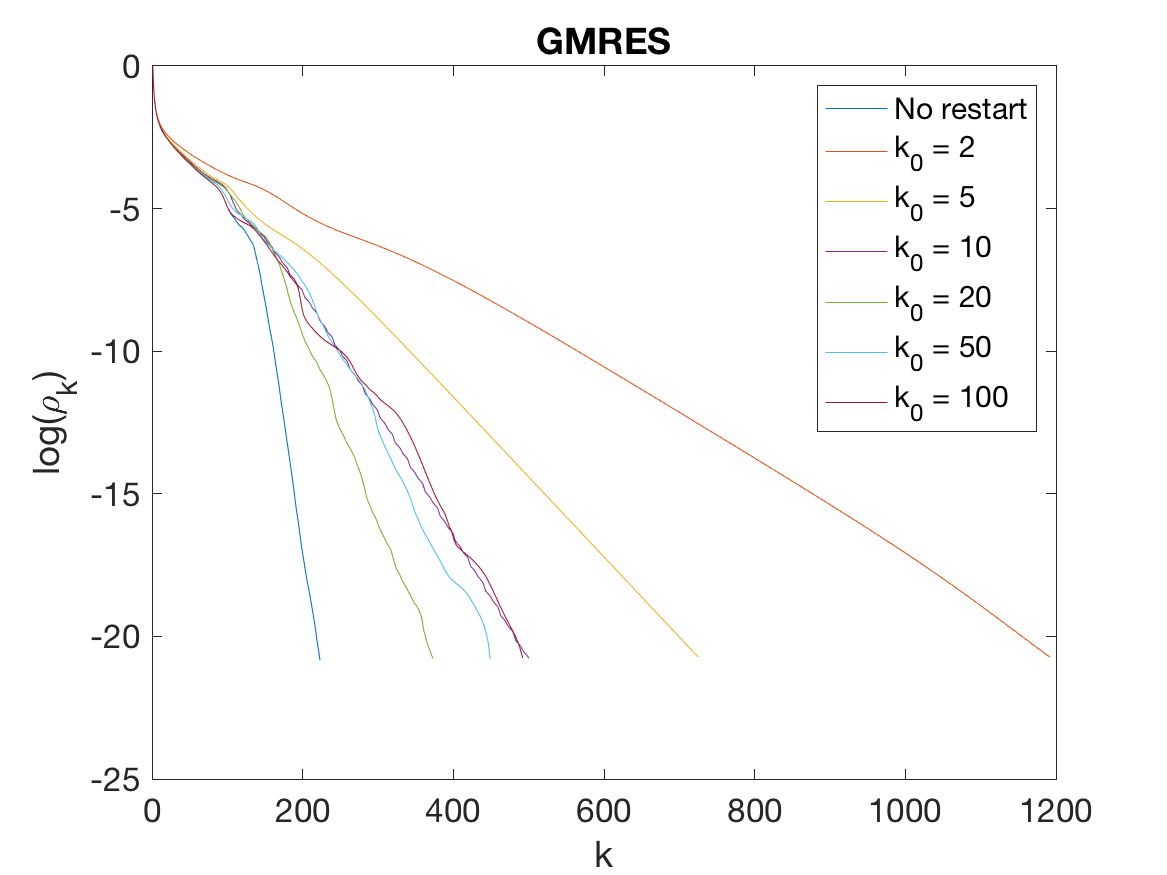
\includegraphics[width=\linewidth]{../Figures/homework4_3.png}
  \begin{center}
    \begin{tabular}{c|c}
      \multicolumn{2}{c}{Matrix-vector products}\\\hline
      \begin{tabular}{l}
        No restart\\
        $k_0=2$\\
        $k_0=5$\\
        $k_0=10$\\
        $k_0=20$\\
        $k_0=50$\\
        $k_0=100$\\
      \end{tabular}
   &$\begin{array}{r}
\texttt{223}\\
\texttt{1787}\\
\texttt{869}\\
\texttt{549}\\
\texttt{391}\\
\texttt{457}\\
\texttt{496}\\
\end{array}
$
    \end{tabular}
  \end{center}
\end{multicols}

\newpage
\newquestion
%======================================================
%
%                    Problem 4
%
%======================================================
\section*{Problem 4}

\newpart
%--------------------------
%    Problem 4 Part A
%--------------------------
\subsection*{(a)}
\begin{eqnarray*}
  A'&=&M_1^{-1}AM_2^{-1}\\
    &=&D\left( D-F\right) ^{-1}\left( D_{0}-F-G\right) \left( D-G\right) ^{-1}\\
    &=&D\left[ \left( D-F\right) ^{-1}\left( \left( Do-2D\right) +\left( D-F\right) +\left( D-G\right) \right) \left( D-G\right) ^{-1}\right] \\
    &=&D\left[ \left( D-F\right) ^{-1}\left( Do-2D\right) \left( D-G\right) ^{-1}+\left( D-G\right) ^{-1}+\left( D-F\right) ^{-1}\right] \\
    &=&D\left( \left( D-G\right) ^{-1}+\left( D-F\right) ^{-1}\left( I+D_{1}\left( D-G\right) ^{-1}\right) \right) 
\end{eqnarray*}

\newpart
%--------------------------
%    Problem 4 Part B
%--------------------------
\subsection*{(b)}
To multiply a vector $q=Av$, we can follow the steps:
\begin{enumerate}
\item Solve $u=\left(D-G\right)^{-1}v$.
\item Multiply $w=D_1u$.
\item Add $x=v+w$.
\item Solve $z=\left(D-F\right)^{-1}x$.
\item Add $p=u+z$.
\item Multiply $q=Dp$.
\end{enumerate}

\newpart
%--------------------------
%    Problem 4 Part C
%--------------------------
\subsection*{(c)}

The two SAXPYs and the two diagonal matrix multiplications each involve $n$ flops. The upper and lower triangular solves require $m$ multiplications and $m$ substractions for each non-diagonal entry and $n$ divisions for a total of $n+2m$. So the total number of flops required is $6n+4m$ flops.

\newpage
\newquestion
%======================================================
%
%                    Problem 5
%
%======================================================
\section*{Problem 5}

\newpart
%--------------------------
%    Problem 5 Part A
%--------------------------
\subsection*{(a)}
\lstinputlisting[style=Matlab-editor,basicstyle=\ttfamily\small]{../Code/gmres_diag.m}
\lstinputlisting[style=Matlab-editor,basicstyle=\ttfamily\small]{../Code/gmres_ssor.m}

\newpage
\newpart
%--------------------------
%    Problem 5 Part B
%--------------------------
\subsection*{(b)}
\lstinputlisting[style=Matlab-editor,basicstyle=\ttfamily\small]{../Code/homework4_5_b_1.m}
\newpage
%=================
% Exmample 1
%=================
For the first matrix with $n=50653$, the code produces the following output:
\begin{multicols}{2}
  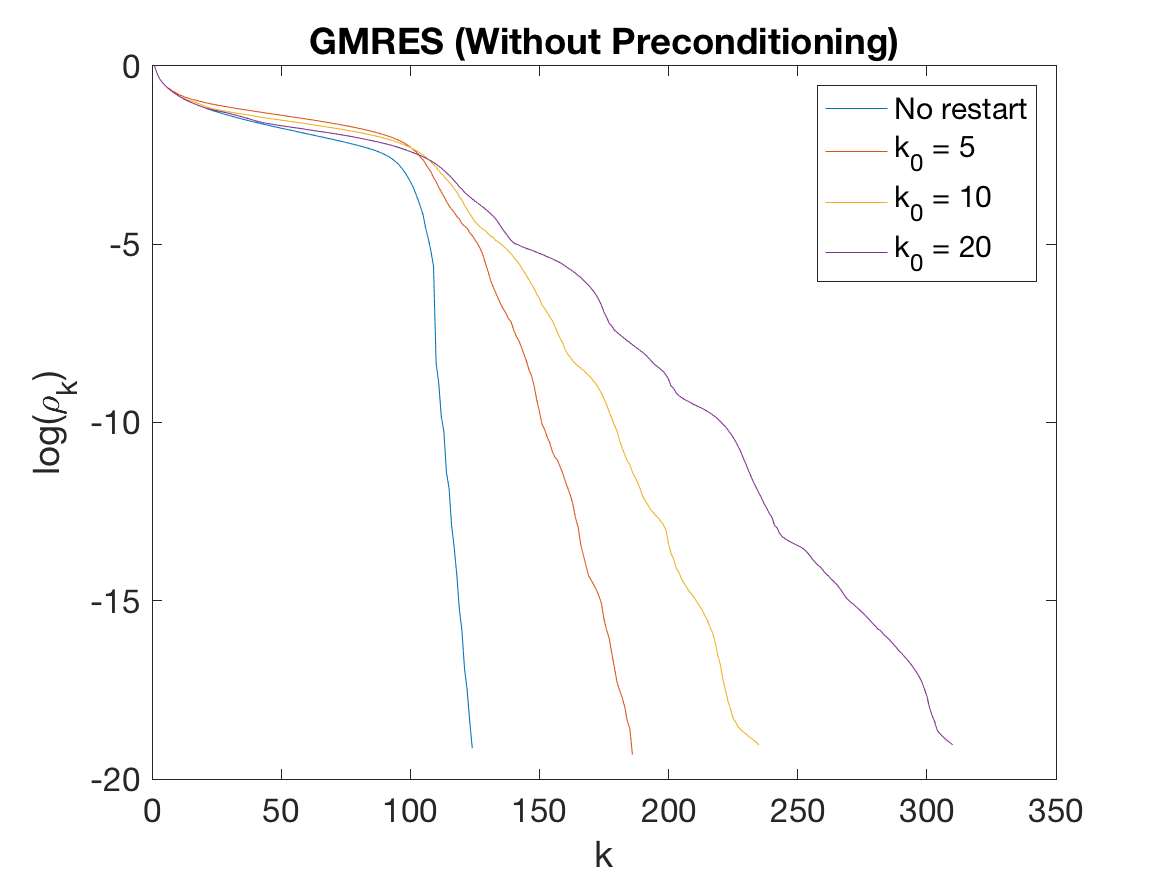
\includegraphics[width=0.8\linewidth]{../Figures/homework4_5_1_default.png}
  \begin{center}
    \begin{tabular}{c|c}
      \multicolumn{2}{c}{Matrix-vector products}\\\hline
      \begin{tabular}{l}
        No restart\\
        $k_0=2$\\
        $k_0=5$\\
        $k_0=10$
      \end{tabular}
   &$\begin{array}{r}
\texttt{124}\\
\texttt{222}\\
\texttt{258}\\
\texttt{325}\\
\end{array}
$
    \end{tabular}
  \end{center}
\end{multicols}
\begin{multicols}{2}
  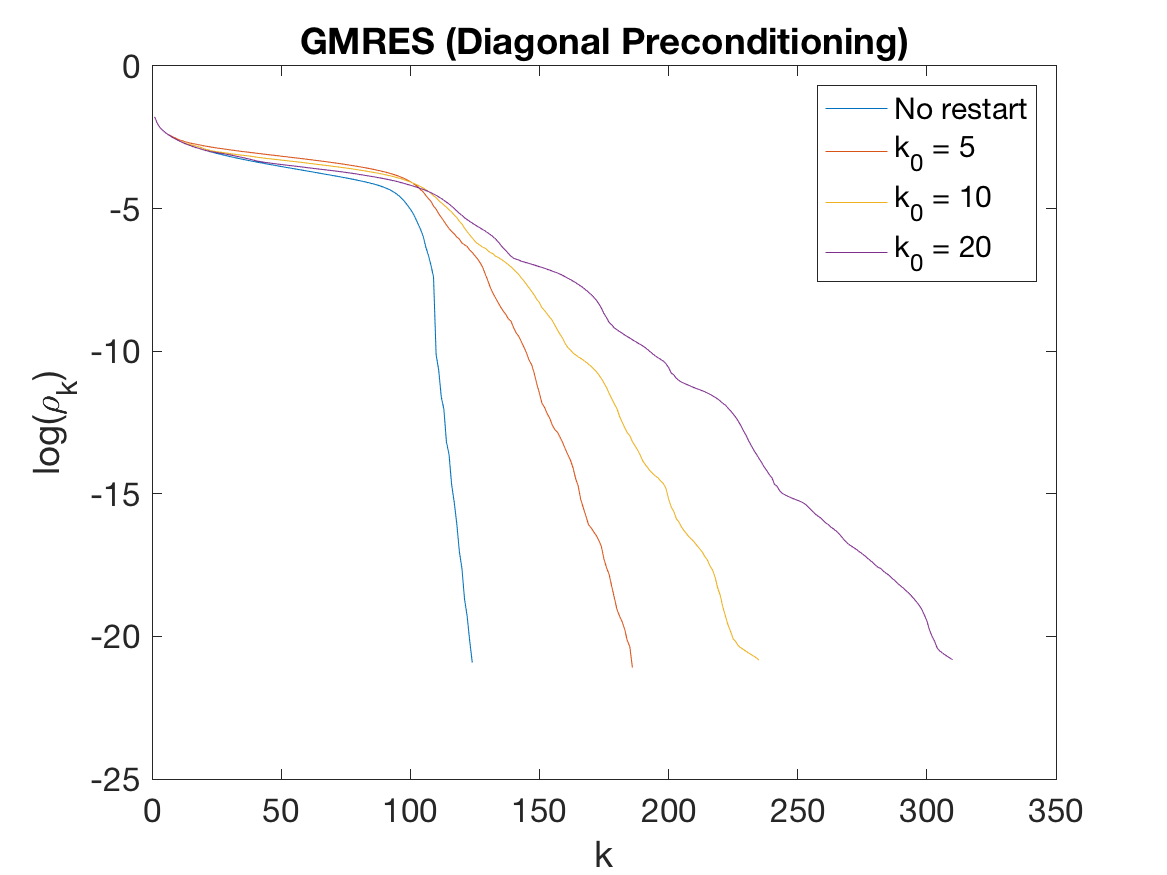
\includegraphics[width=0.8\linewidth]{../Figures/homework4_5_1_diag.png}
  \begin{center}
    \begin{tabular}{c|c}
      \multicolumn{2}{c}{Matrix-vector products}\\\hline
      \begin{tabular}{l}
        No restart\\
        $k_0=2$\\
        $k_0=5$\\
        $k_0=10$
      \end{tabular}
   &$\begin{array}{r}
\texttt{124}\\
\texttt{222}\\
\texttt{258}\\
\texttt{325}\\
\end{array}
$
    \end{tabular}
  \end{center}
\end{multicols}
\begin{multicols}{2}
  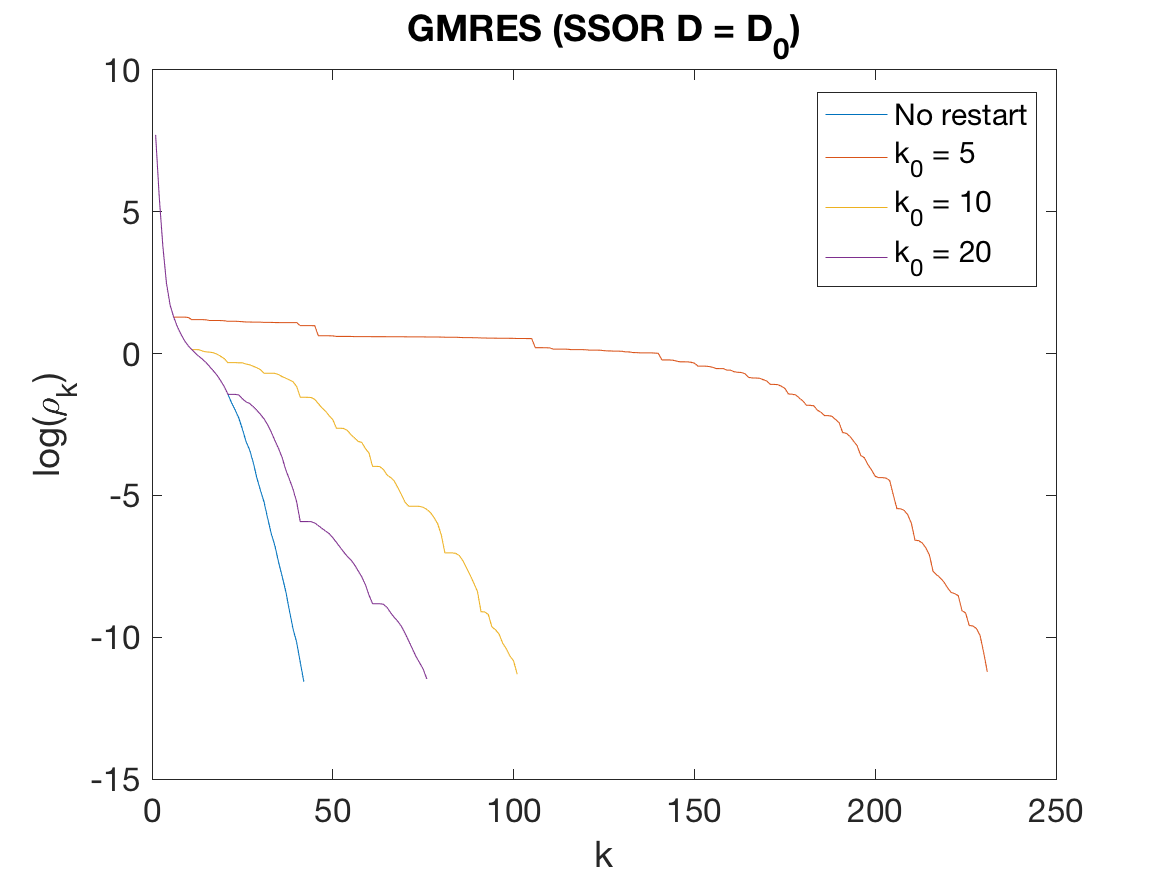
\includegraphics[width=0.8\linewidth]{../Figures/homework4_5_1_ssordiag.png}
  \begin{center}
    \begin{tabular}{c|c}
      \multicolumn{2}{c}{Matrix-vector products}\\\hline
      \begin{tabular}{l}
        No restart\\
        $k_0=2$\\
        $k_0=5$\\
        $k_0=10$
      \end{tabular}
   &$\begin{array}{r}
\texttt{42}\\
\texttt{276}\\
\texttt{110}\\
\texttt{79}\\
\end{array}
$
    \end{tabular}
  \end{center}
\end{multicols}
\begin{multicols}{2}
  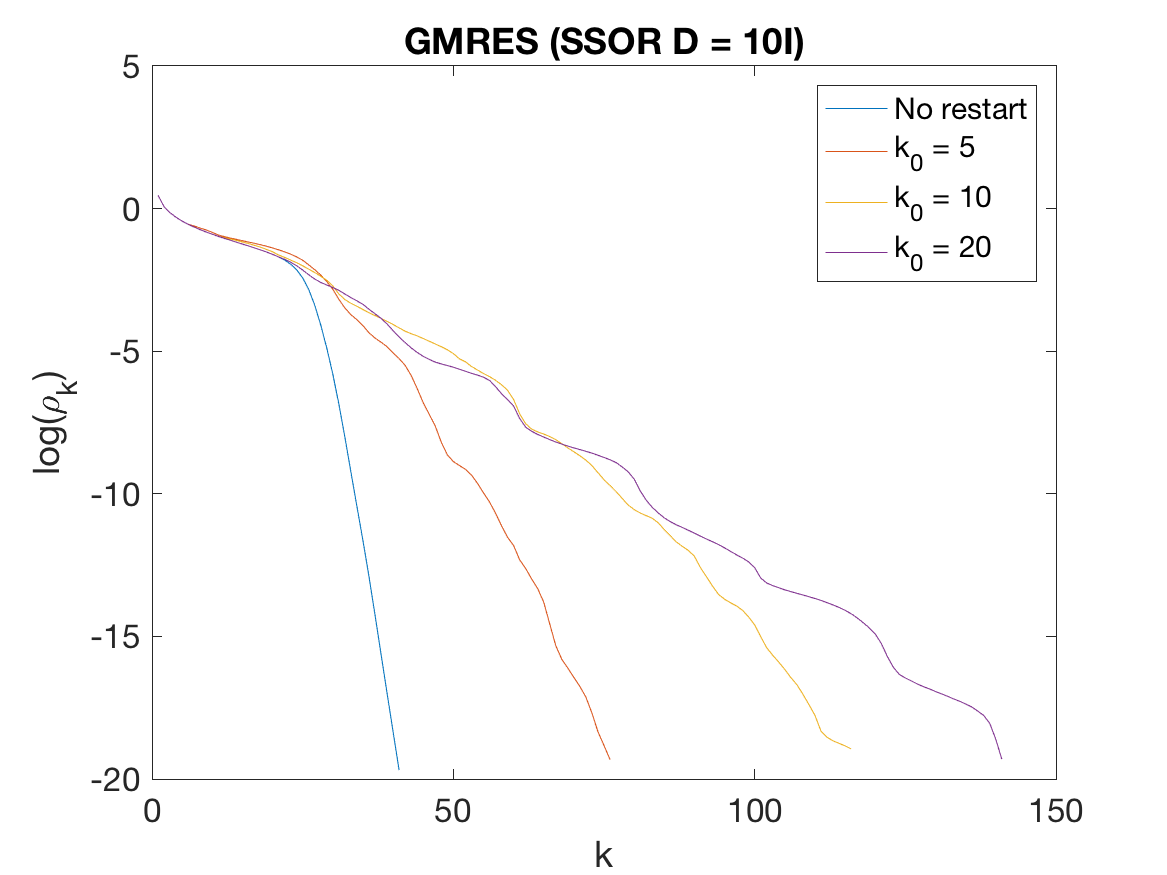
\includegraphics[width=0.8\linewidth]{../Figures/homework4_5_1_ssoriden.png}
  \begin{center}
    \begin{tabular}{c|c}
      \multicolumn{2}{c}{Matrix-vector products}\\\hline
      \begin{tabular}{l}
        No restart\\
        $k_0=2$\\
        $k_0=5$\\
        $k_0=10$
      \end{tabular}
   &$\begin{array}{r}
\texttt{41}\\
\texttt{90}\\
\texttt{127}\\
\texttt{147}\\
\end{array}
$
    \end{tabular}
  \end{center}
\end{multicols}
\newpage
%=================
% Exmample 2
%=================
For the first matrix with $n=389017$, the code produces the following output:
\begin{multicols}{2}
  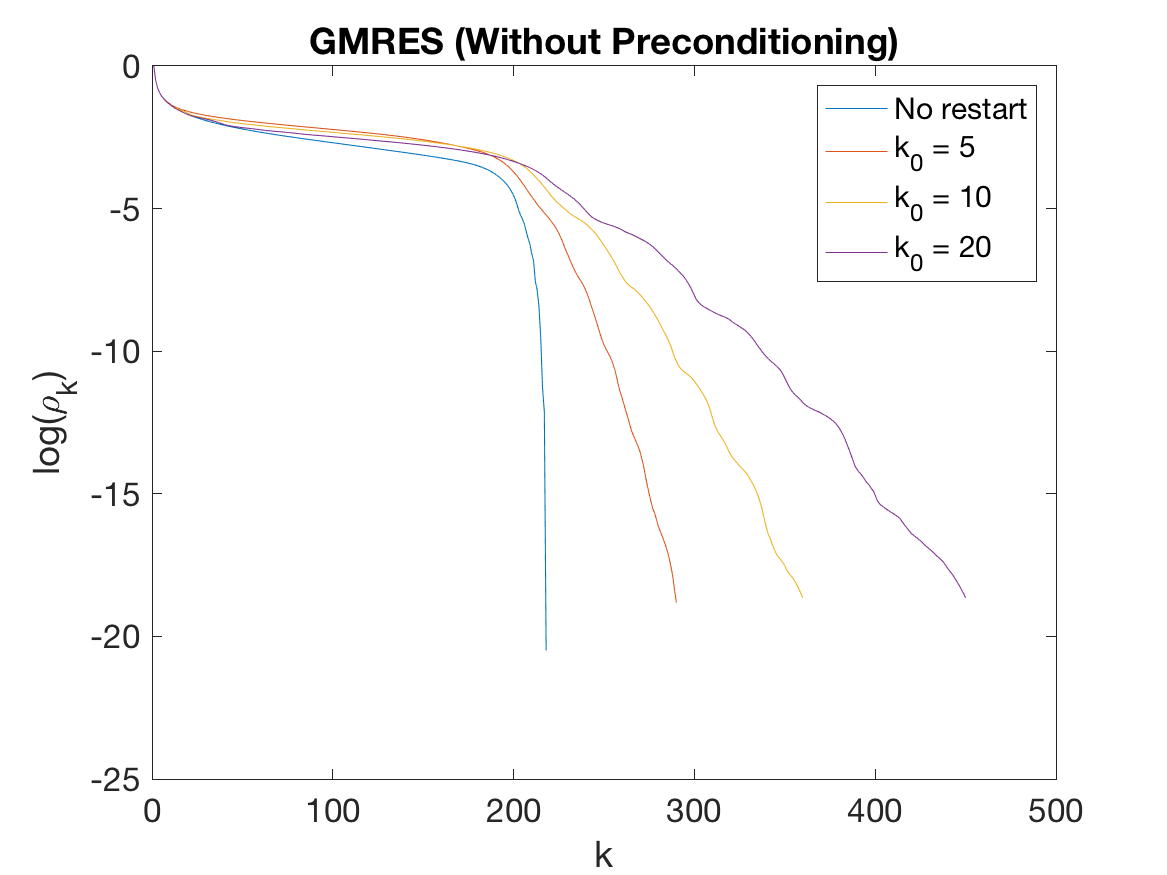
\includegraphics[width=0.8\linewidth]{../Figures/homework4_5_2_default.png}
  \begin{center}
    \begin{tabular}{c|c}
      \multicolumn{2}{c}{Matrix-vector products}\\\hline
      \begin{tabular}{l}
        No restart\\
        $k_0=2$\\
        $k_0=5$\\
        $k_0=10$
      \end{tabular}
   &$\begin{array}{r}
\texttt{218}\\
\texttt{347}\\
\texttt{395}\\
\texttt{472}\\
\end{array}
$
    \end{tabular}
  \end{center}
\end{multicols}
\begin{multicols}{2}
  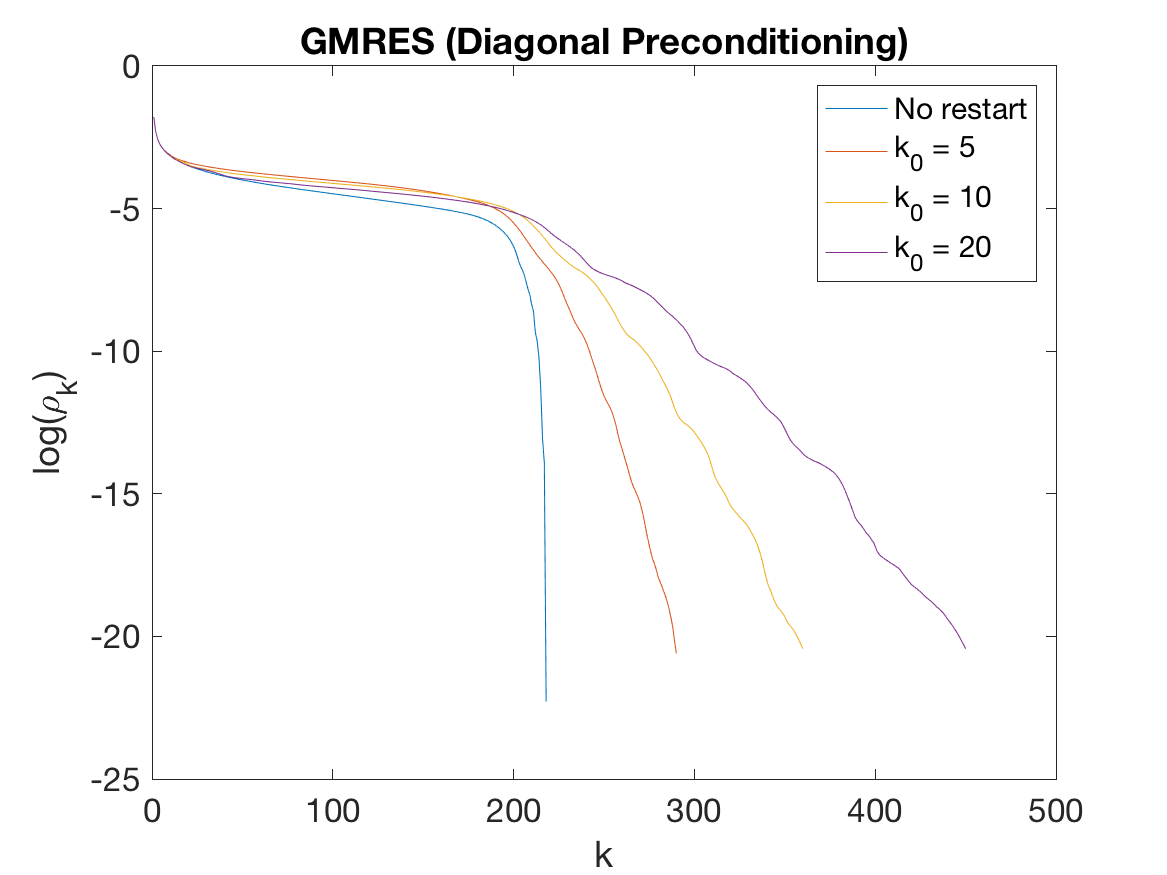
\includegraphics[width=0.8\linewidth]{../Figures/homework4_5_2_diag.png}
  \begin{center}
    \begin{tabular}{c|c}
      \multicolumn{2}{c}{Matrix-vector products}\\\hline
      \begin{tabular}{l}
        No restart\\
        $k_0=2$\\
        $k_0=5$\\
        $k_0=10$
      \end{tabular}
   &$\begin{array}{r}
\texttt{218}\\
\texttt{347}\\
\texttt{395}\\
\texttt{472}\\
\end{array}
$
    \end{tabular}
  \end{center}
\end{multicols}
\begin{multicols}{2}
  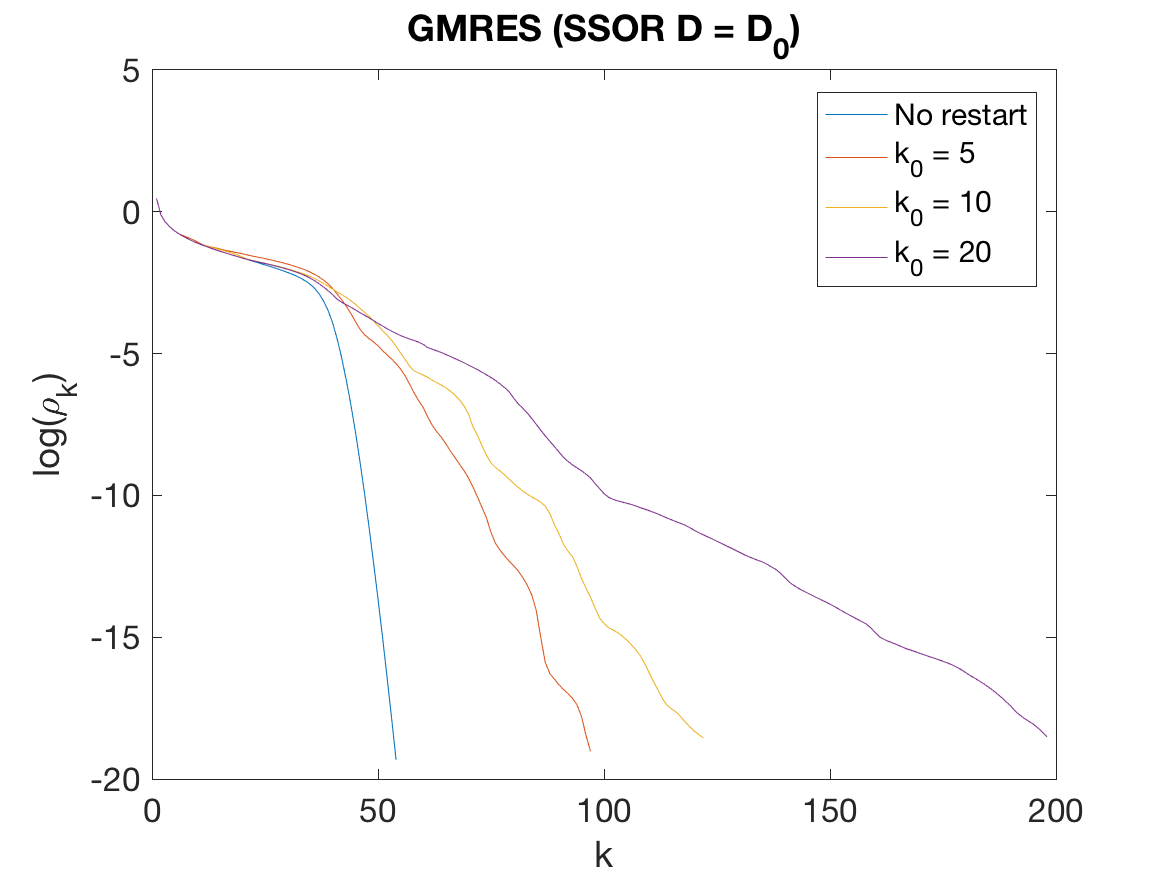
\includegraphics[width=0.8\linewidth]{../Figures/homework4_5_2_ssordiag.png}
  \begin{center}
    \begin{tabular}{c|c}
      \multicolumn{2}{c}{Matrix-vector products}\\\hline
      \begin{tabular}{l}
        No restart\\
        $k_0=2$\\
        $k_0=5$\\
        $k_0=10$
      \end{tabular}
   &$\begin{array}{r}
\texttt{54}\\
\texttt{116}\\
\texttt{134}\\
\texttt{207}\\
\end{array}
$
    \end{tabular}
  \end{center}
\end{multicols}
\begin{multicols}{2}
  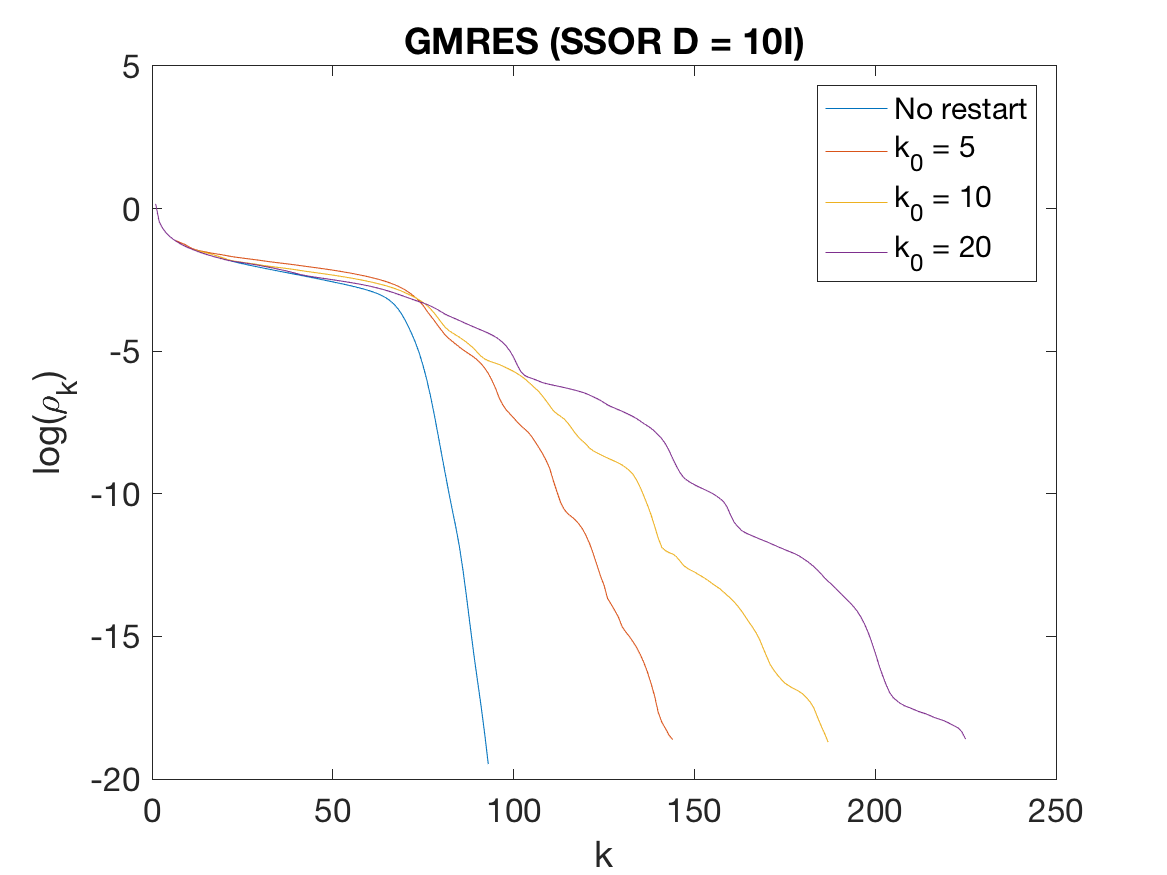
\includegraphics[width=0.8\linewidth]{../Figures/homework4_5_2_ssoriden.png}
  \begin{center}
    \begin{tabular}{c|c}
      \multicolumn{2}{c}{Matrix-vector products}\\\hline
      \begin{tabular}{l}
        No restart\\
        $k_0=2$\\
        $k_0=5$\\
        $k_0=10$
      \end{tabular}
   &$\begin{array}{r}
\texttt{93}\\
\texttt{172}\\
\texttt{205}\\
\texttt{236}\\
\end{array}
$
    \end{tabular}
  \end{center}
\end{multicols}

\end{document}
%================================================================
%================================================================
%
%                           Templates
%
%================================================================
%================================================================


%----------------------------------------------------------------
%----------------------------------------------------------------


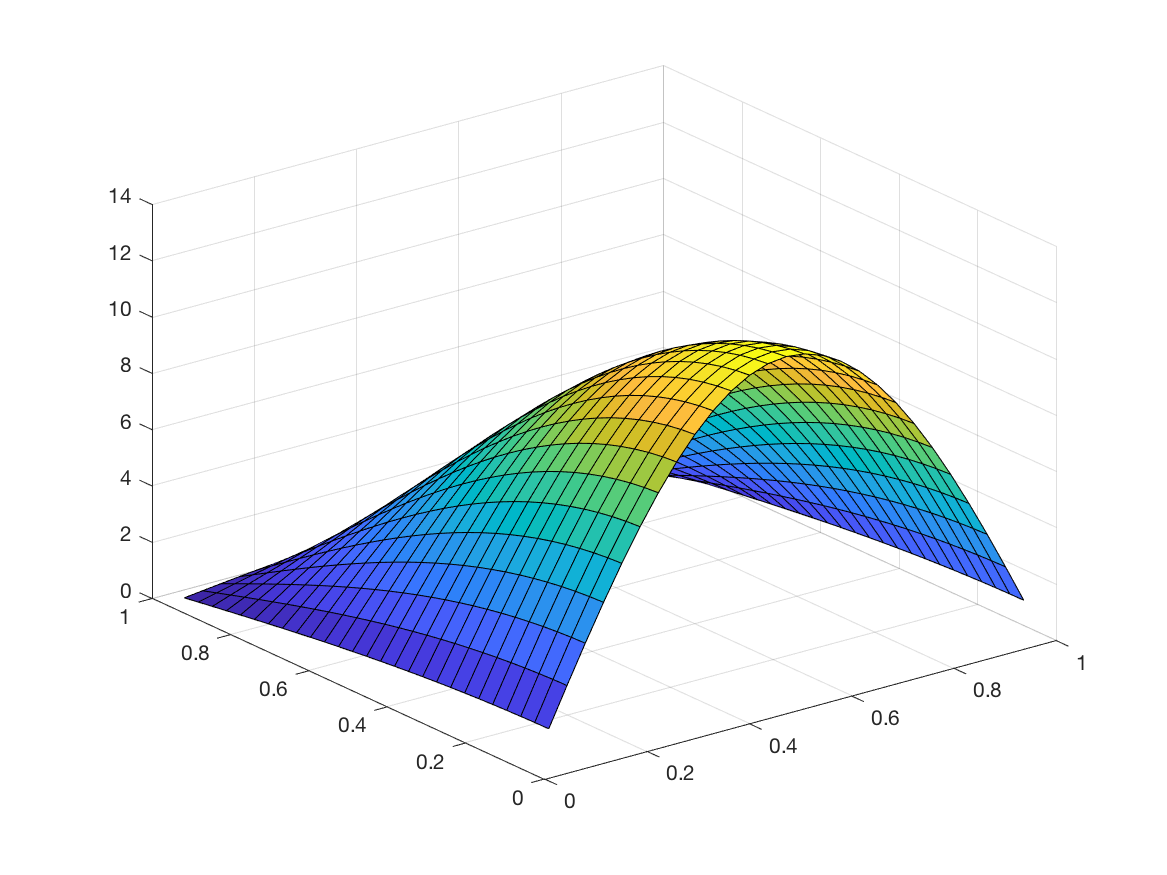
\includegraphics[width=\linewidth]{../Figures/poisson_rhs_1.png}
\lstinputlisting[style=Matlab-editor,basicstyle=\ttfamily\small]{../Code/solvePoisson.m}

\newquestion
%======================================================
%
%                    Problem n
%
%======================================================
\section*{Problem n}

\newpart
%--------------------------
%    Problem n Part A
%--------------------------
\subsection*{(a)}

\newpart
%--------------------------
%    Problem n Part B
%--------------------------
\subsection*{(b)}


%----------------------------------------------------------------
%----------------------------------------------------------------


%======================================================
%
%               Appendix: Problem n
%
%======================================================
%--------------------------
%  Appendix: P n Part A
%--------------------------
\subsection*{Problem n Part A}

\newpage
%--------------------------
%  Appendix: P n Part B
%--------------------------
\subsection*{Problem n Part B}


%----------------------------------------------------------------
%----------------------------------------------------------------